%% -----------------------------------------------------------------
%% Tether_Grace — Graduate Reference and Case Study
%% Comprehensive reference for re-creating the system
%% -----------------------------------------------------------------
\documentclass[11pt,a4paper,oneside]{report}

%% ---- packages -------------------------------------------------
\usepackage[T1]{fontenc}
\usepackage[utf8]{inputenc}
\IfFileExists{lmodern.sty}{\usepackage{lmodern}}{} % optional — fallback to CM
% microtype intentionally omitted: requires scalable fonts that may be absent
% on minimal TeX Live installs. Compile result is unaffected.
\usepackage[margin=1in]{geometry}
\usepackage{amsmath, amssymb, amsthm, mathtools}
\usepackage{siunitx}  % \SI{...}{...} used in methods/results sections
\usepackage{empheq}   % \begin{empheq}[box=...]{equation}
\usepackage{bm}
\usepackage{booktabs}
\usepackage{array}
\usepackage{longtable}
\usepackage{enumitem}
\usepackage{graphicx}
\usepackage{xcolor}
\usepackage[most]{tcolorbox}
\usepackage{listings}
\usepackage{hyperref}
\usepackage{cleveref}
\usepackage{fancyhdr}
\usepackage{titlesec}
\usepackage{tikz}
\usetikzlibrary{arrows.meta, positioning, shapes.geometric, calc, decorations.pathreplacing}

%% ---- hyperref / cross-refs ------------------------------------
\hypersetup{
  colorlinks=true,
  linkcolor=blue!60!black,
  citecolor=green!60!black,
  urlcolor=magenta!60!black,
  pdftitle={Tether_Grace Graduate Reference},
  pdfauthor={Tether_Grace Project},
  pdfsubject={Decentralized Fault-Tolerant Cooperative Aerial Payload Transport}
}

%% ---- code listing style ---------------------------------------
\definecolor{codebg}{rgb}{0.97,0.97,0.97}
\definecolor{codekw}{rgb}{0.13,0.29,0.53}
\definecolor{codecom}{rgb}{0.40,0.40,0.40}
\definecolor{codestr}{rgb}{0.60,0.20,0.20}
\lstdefinestyle{cpp}{
  language=C++,
  basicstyle=\small\ttfamily,
  keywordstyle=\color{codekw}\bfseries,
  commentstyle=\color{codecom}\itshape,
  stringstyle=\color{codestr},
  numbers=left, numberstyle=\tiny\color{gray},
  backgroundcolor=\color{codebg},
  frame=single, rulecolor=\color{gray!50},
  breaklines=true, showstringspaces=false,
  tabsize=2, captionpos=b
}
\lstdefinestyle{shell}{
  basicstyle=\small\ttfamily,
  backgroundcolor=\color{codebg},
  frame=single, rulecolor=\color{gray!50},
  breaklines=true, showstringspaces=false, tabsize=2,
  morecomment=[l]{\#},
  commentstyle=\color{codecom}\itshape
}
\lstset{style=cpp}

%% ---- custom math macros ---------------------------------------
\newcommand{\rope}{\text{rope}}
\newcommand{\bx}{\bm{x}}
\newcommand{\bp}{\bm{p}}
\newcommand{\bv}{\bm{v}}
\newcommand{\ba}{\bm{a}}
\newcommand{\bs}{\bm{s}}
\newcommand{\bu}{\bm{u}}
\newcommand{\bF}{\bm{F}}
\newcommand{\btau}{\bm{\tau}}
\newcommand{\bomega}{\bm{\omega}}
\newcommand{\be}{\bm{e}}
\newcommand{\R}{\mathbb{R}}
\newcommand{\SO}{\mathrm{SO}}
\newcommand{\diag}{\mathrm{diag}}
\newcommand{\sat}{\mathrm{sat}}

%% ---- evidence-tag boxes ---------------------------------------
\newtcolorbox{evidence}[1]{
  colback=yellow!5!white, colframe=yellow!60!black,
  boxrule=0.4pt, arc=1mm, left=2mm, right=2mm,
  title=#1, fonttitle=\bfseries\small, coltitle=black,
  breakable
}
\newtcolorbox{insight}[1]{
  colback=blue!4!white, colframe=blue!40!black,
  boxrule=0.4pt, arc=1mm, left=2mm, right=2mm,
  title=#1, fonttitle=\bfseries\small, coltitle=black,
  breakable
}
\newtcolorbox{warning}[1]{
  colback=red!4!white, colframe=red!40!black,
  boxrule=0.4pt, arc=1mm, left=2mm, right=2mm,
  title=#1, fonttitle=\bfseries\small, coltitle=black,
  breakable
}
\newcommand{\Obs}{\textcolor{green!50!black}{\textbf{[O]}}}
\newcommand{\Der}{\textcolor{blue!60!black}{\textbf{[D]}}}
\newcommand{\Inf}{\textcolor{orange!70!black}{\textbf{[I]}}}
\newcommand{\Emp}{\textcolor{purple!60!black}{\textbf{[E]}}}
\newcommand{\Lim}{\textcolor{red!60!black}{\textbf{[L]}}}

%% ---- headers --------------------------------------------------
\pagestyle{fancy}
\fancyhf{}
\fancyhead[R]{\small\leftmark}
\fancyhead[L]{\small Tether\_Grace Reference}
\fancyfoot[C]{\thepage}
\renewcommand{\headrulewidth}{0.4pt}

%% ---- title ----------------------------------------------------
\title{%
  \huge\textbf{Tether\_Grace}\\[0.4em]
  \Large A Case Study in Decentralized Fault-Tolerant\\
  Cooperative Aerial Payload Transport \\[0.8em]
  \large\emph{Graduate Reference and Reproducibility Companion}
}
\author{Tether\_Grace Project Team}
\date{\today}

%% =================================================================
\begin{document}
\maketitle

\thispagestyle{empty}
\begin{abstract}
Four quadrotors cooperatively lift a 3~kg payload suspended on four
cables in an underslung sling configuration. At any instant during a
25--40~s trajectory, a cable can be severed. Each quadrotor runs an
identical \emph{fully-local} controller whose only inputs are its own
rigid-body state, its own rope's scalar tension, the (locally
observable) payload state, and a \emph{shared feed-forward}
reference trajectory. There is no peer-drone state exchange, no
\emph{N-alive} estimator, no centralised fault flag. At every control
step each drone solves a three-variable convex quadratic program that
jointly minimises (i) formation-slot tracking error, (ii) payload
pendulum swing, and (iii) control effort, subject to tilt-envelope
and thrust-envelope constraints. The fault-tolerance behaviour is
\emph{emergent}: when a peer's cable severs, the payload redistributes
its load through the surviving ropes and the surviving drones'
tension feed-forward automatically increases to compensate---no
inter-drone messaging of any kind.

This document is a self-contained graduate reference. It derives the
full multibody-rope system model, presents the controller design
with equation-to-code cross-references, explains the Drake simulation
infrastructure with enough implementation detail to re-create it,
reports the six-scenario validation campaign, and closes with a
discussion of novelty, limitations, and student-scaled extensions.
Every load-bearing numerical claim is tagged with its evidence
status: \Obs~observed in code or log, \Der~derived on paper from
observed quantities, \Inf~high-confidence inference, \Emp~empirical
only (no proof), or \Lim~explicit limitation.
\end{abstract}

%% ---- TOC ------------------------------------------------------
\tableofcontents
\clearpage

%% ===============================================================
\chapter*{Preface}
\addcontentsline{toc}{chapter}{Preface}

\section*{Who this document is for}

You are a graduate student in robotics and/or control. You are
comfortable with Newton--Euler rigid-body dynamics, state-space
representations, pole placement, and convex optimisation (LP/QP). You
have heard of Drake but possibly never written a \texttt{LeafSystem}.
You want a complete reference for a simulated cooperative-lift
system that you could re-implement from scratch after reading.

\section*{How to read it}

The book is organised in six parts. Parts~I and II set up the
physical problem and derive the multibody and rope models. Part~III
specifies the control problem and constructs the fully-local QP
controller. Part~IV covers the Drake implementation, including the
code architecture and the signal wiring. Part~V is the validation
campaign and its results. Part~VI discusses what is novel, what is
textbook, and what remains open. The appendices (\Cref{chap:params},
\Cref{chap:code-map}, \Cref{chap:reproduce}, \Cref{chap:exercises},
\Cref{chap:evidence}) are reference material.

\section*{Evidence tags}

Every substantive numerical or structural claim is tagged with one of
\Obs, \Der, \Inf, \Emp, or \Lim. The definitions are in the abstract;
the full audit log is in \Cref{chap:evidence}.

\section*{Code and source references}

Paths such as
\texttt{decentralized\_local\_controller.cc:L199} point into the
companion repository. The document tracks the state of the code in
the top-level commit of the accompanying tree.

%% ===============================================================
\part{Problem Formulation}
%% ===============================================================

\chapter{Introduction}
\label{chap:intro}

\section{Motivation}

Cooperative aerial manipulation of heavy payloads with multiple
multirotors is a recurring problem in aerial logistics, search and
rescue, and outdoor robotics. A single multirotor is limited by its
thrust; cooperation turns $N$ lighter drones into an effective
lifter of a payload up to roughly $N\times$ the single-drone capacity.
Cable slings are the standard mechanical interface: cheap, light,
tolerant to small geometric disagreements, and deterministic
(ropes cannot push, only pull).

The price of this configuration is underactuation and coupling. The
payload hanging from multiple cables behaves as a pendulum whose
mode couples into every drone's position loop. When one cable
severs---a non-trivial failure mode, since cables chafe, fatigue, or
get cut by debris---the remaining drones must rebalance the load
fast enough to keep the payload airborne.

\section{Related work}

Single-drone cable-suspended transport is textbook material
\cite{Sreenath2013, Lee2010, Palunko2012}. The multi-drone cooperative
case has been studied in numerous variants: rigid-bar payloads
\cite{Lee2018}, centralised MPC over the full system
\cite{Wehbeh2021}, leader--follower architectures, and consensus-based
distributed controllers. The prevailing thread is that fault tolerance
requires either (i) centralised re-planning, (ii) an explicit
fault-detection module on every drone, or (iii) a peer-state
consensus protocol. None of these is essential for the problem,
as we show below.

\section{Contributions}
\label{sec:contributions}

\begin{enumerate}
\item A \emph{fully-local} controller: each drone sees only its own
state, its own rope tension, the payload state, and a shared
feed-forward reference. No peer-drone information, no fault flag,
no consensus protocol.
\item A \emph{per-step convex QP} (three decision variables) that
jointly encodes tracking, pendulum-swing damping, and control-effort
minimisation, with hard tilt- and thrust-envelope constraints.
\item A demonstration that \emph{cable-severance fault tolerance
emerges from the coupled physics} alone: when a peer fails, the
payload redistributes load onto the surviving ropes, each survivor's
rope-tension measurement rises, its tension feed-forward rises,
and the payload is caught. No explicit inter-drone signal is
exchanged at any point.
\item A reproducible six-scenario simulation campaign in Drake,
covering nominal straight traverse, single/dual/triple sequential
cable severance, and fault-during-figure-8 manoeuvre. Numerical
results are reported end-to-end; every artefact is a deterministic
output of a single runner script.
\end{enumerate}

\begin{insight}{What this document is \emph{not}}
It is not a proof of closed-loop stability under cable severance:
that proof is open (see \Cref{chap:discussion}). It is also not a
hardware report: every claim in this document is a simulation result
(\Lim).
\end{insight}

\chapter{Problem Statement}
\label{chap:problem}

\section{System and reference}

Consider $N=4$ quadrotors $\{Q_i\}_{i=0}^{3}$ and a payload $L$ of mass
$m_L$. Each quadrotor is connected to the payload by an independent
cable of rest length $L$. The mission specifies a time-parameterised
payload reference trajectory $\bar{\bp}_L(t) \in \R^3$,
$\bar{\bv}_L(t) \in \R^3$ over $t\in[0,T]$, known to every drone as a
feed-forward signal.

\section{Signals available to each drone}

Drone~$i$'s controller reads, at every control step:

\begin{longtable}{>{\ttfamily}p{0.30\textwidth} p{0.40\textwidth} p{0.22\textwidth}}
\toprule
\textbf{Signal} & \textbf{Meaning} & \textbf{Source} \\
\midrule
p\_self, v\_self & own pose and velocity $(\bp_i, \bv_i)$ & plant state port \\
R\_self, omega\_W & own attitude $R_i$ and body angular velocity $\bomega_i$ & plant state port \\
T\_i & scalar top-segment rope tension & \texttt{RopeForceSystem}'s tension output \\
p\_L, v\_L & payload pose and velocity $(\bp_L, \bv_L)$ & onboard IR range sensor (ground-truth in simulation) \\
$\bar{\bp}_L(t), \bar{\bv}_L(t)$ & shared payload reference & mission planner (feed-forward only) \\
\bottomrule
\end{longtable}

Signals \emph{not} available to drone~$i$'s controller:

\begin{itemize}
\item State of any other drone.
\item Tension on any other rope.
\item Fault flag / severance notification / \emph{N-alive} count.
\item Accelerometer / IMU output of the payload beyond what the rope
tension reveals.
\end{itemize}

\section{Fault model}

A cable-severance fault at time $t_{\text{fault}}$ instantaneously
zeros the $i$-th rope's force on all endpoints (drone, beads,
payload). The fault time is known to the simulation; in a real
deployment a small detector on the faulted drone would estimate it
from its own tension signal (see \Cref{sec:fault-open}).

\section{Performance requirements}

\begin{enumerate}
\item Payload position tracks $\bar{\bp}_L(t)$ with bounded RMS error.
\item All rope tensions remain positive and finite.
\item All rotor thrusts and body torques remain within their
envelopes.
\item Under any cable-severance sequence, the payload remains
airborne---no rope overload, no drone ground collision, no
pathological oscillation.
\end{enumerate}

\section{Research question}

\begin{center}
\emph{How do we control a fleet of quadrotors carrying an under-slung
payload, using only local information per drone, while tolerating
arbitrary cable-severance faults without explicit fault signalling?}
\end{center}

%% ===============================================================
\part{Mathematical Foundations}
%% ===============================================================

\chapter{Multibody Dynamics}
\label{chap:dynamics}

We model the plant as a standard Newton--Euler multibody system and
integrate it with Drake's \texttt{MultibodyPlant}. This chapter
states the equations and maps them to the simulator's state.

\section{Quadrotor rigid-body dynamics}

\noindent Each drone $Q_i$ is a rigid body with mass $m_i=1.5$~kg and
inertia $J_i$ (computed by Drake from the URDF geometry). Its
Newton--Euler equations in the world frame are

\begin{equation}
\dot{\bp}_i = \bv_i, \qquad
m_i\, \dot{\bv}_i = R_i\, \be_3\, f_i + \bF_{\rope,i} - m_i g\, \be_3,
\label{eq:drone-trans}
\end{equation}

\begin{equation}
\dot{R}_i = R_i\, \widehat{\bomega}_i^{B}, \qquad
J_i\, \dot{\bomega}_i^{B} + \bomega_i^{B}\times J_i\bomega_i^{B} = \btau_i,
\label{eq:drone-rot}
\end{equation}

where $\be_3=(0,0,1)^\top$, $R_i\in\SO(3)$, $\widehat{\cdot}$ is the
skew-symmetric map, $f_i\ge 0$ is the scalar body-z thrust,
$\btau_i\in\R^3$ is the body-frame torque, and
$\bF_{\rope,i}\in\R^3$ is the world-frame force that rope~$i$ applies
at the drone's attachment point.

\begin{evidence}{Evidence}
\Obs. Drake \texttt{MultibodyPlant}'s built-in rigid-body dynamics
implements \Cref{eq:drone-trans,eq:drone-rot}. The controller emits
$(\,\btau_i, R_i\be_3 f_i\,)$ as an
\texttt{ExternallyAppliedSpatialForce} at the drone body. Rotor
dynamics are not modelled (\Lim).
\end{evidence}

\section{Payload dynamics}

The payload is a solid sphere of mass $m_L=3$~kg and radius
$r_L=0.15$~m, with inertia $J_L = \frac{2}{5}m_L r_L^2 I$. It has no
thrust input; only rope forces and gravity act on it:

\begin{equation}
m_L\, \dot{\bv}_L = \sum_{j=1}^{N} \bF_{\rope,j}^{(L)} - m_L g\, \be_3,
\label{eq:payload-trans}
\end{equation}
\begin{equation}
J_L\, \dot{\bomega}_L^{B} + \bomega_L^{B}\times J_L\bomega_L^{B}
= \sum_{j=1}^{N} \bm{r}_{j,L}\times R_L^{\!\top}\bF_{\rope,j}^{(L)},
\label{eq:payload-rot}
\end{equation}

where $\bF_{\rope,j}^{(L)}$ is the payload-side force of rope~$j$ and
$\bm{r}_{j,L}$ is the attachment offset in the payload body frame.

\section{Coupled plant state}

The full system consists of $N$ drones plus one payload plus $N\times
N_{\text{seg}}$ internal rope beads (see \Cref{chap:rope}). Each
rigid body contributes 7 positional coordinates (3 position + 4
quaternion) and 6 velocity coordinates, so the total plant state has
dimension
\begin{equation}
\dim\,\mathbf{x}_\text{plant}
= (N + 1 + N\cdot N_{\text{seg}})\cdot(7+6) = (4+1+32)\cdot 13 = 481.
\end{equation}

\Der. Integrator is Drake's implicit-Euler discrete-time stepper at
$\Delta t = 2\times 10^{-4}$~s.

\chapter{Bead-Chain Cable Model}
\label{chap:rope}

\section{Discretisation}

Each rope is modelled as a chain of $N_{\text{seg}}=8$ point-mass
beads connected by spring-damper segments. The beads are full rigid
bodies in the plant; each has mass $m_b=0.025$~kg and solid-sphere
inertia.

Let $\bx_{i,k}$, $k=0,\ldots,N_{\text{seg}}$, denote the world position
of the $k$-th node of rope $i$; $\bx_{i,0}$ is the drone attachment
point and $\bx_{i,N_{\text{seg}}}$ is the payload attachment. Segment
$k$ has rest length
\begin{equation}
L_\text{seg} = L / N_{\text{seg}}.
\end{equation}

\section{Per-segment force law}

Define unit vector, length, stretch, and stretch rate of segment
$k$:
\begin{align}
\hat{\bu}_{i,k} &= \frac{\bx_{i,k}-\bx_{i,k-1}}{\|\bx_{i,k}-\bx_{i,k-1}\|}, \\
\ell_{i,k} &= \|\bx_{i,k}-\bx_{i,k-1}\|, \\
\Delta_{i,k} &= \ell_{i,k} - L_\text{seg}, \\
\dot{\ell}_{i,k} &= \hat{\bu}_{i,k}^{\!\top}(\dot{\bx}_{i,k}-\dot{\bx}_{i,k-1}).
\end{align}

The segment tension is a \emph{tension-only Kelvin--Voigt} law:

\begin{empheq}[box=\tcbhighmath]{equation}
T_{i,k} = \max\!\Big(\, 0,\;\; k_s\,\Delta_{i,k} + c_s\,\dot{\ell}_{i,k}\,\Big).
\label{eq:segment-tension}
\end{empheq}

The outer $\max$ captures the essential physical property that a
cable can only pull, not push. Equal and opposite forces
$\pm T_{i,k}\hat{\bu}_{i,k}$ are applied at the two endpoints.

\Obs. Parameters are $k_s=25\,000$~N/m and $c_s=60$~N$\cdot$s/m
(\texttt{decentralized\_fault\_aware\_sim\_main.cc}).

\section{End-to-end effective stiffness}

Treating the chain as $N_{\text{seg}}$ springs in series,
\begin{equation}
k_{\rope}^{\text{eff}} = \frac{k_s}{N_{\text{seg}}}
= \frac{25\,000}{8} = 3\,125~\text{N/m}.
\label{eq:keff}
\end{equation}

\Der. At cruise the per-rope tension is
$m_L g/N = 3\cdot 9.81/4 = 7.36$~N, so the static stretch is
$\Delta L_\text{cruise}\approx 7.36/3125 \approx 2.4$~mm---
effectively rigid.

\section{Damping and stability bound}

The bead-level natural frequency is
\begin{equation}
\omega_n^{\text{seg}} = \sqrt{k_s/m_b} = \sqrt{25\,000/0.025}
\approx 1\,000~\text{rad/s}. \label{eq:omega-seg}
\end{equation}

The bead-level damping ratio is
\begin{equation}
\zeta = \frac{c_s}{2\sqrt{k_s m_b}} \approx 1.2,
\end{equation}
slightly overdamped: no ringing.

An explicit-Euler stability bound is
$\Delta t_\text{stable} < 2/\omega_n^{\text{seg}} \approx 2$~ms.
Drake's implicit-Euler and $\Delta t = 0.2$~ms leave a $\sim 10\times$
safety margin.

\section{Catenary drape}

For a formation-centred, statically-taut rope of length $L$ with
drone at horizontal offset $r_f$, the straight-line drone-to-payload
distance is
\begin{equation}
d^{\text{taut}} = \sqrt{L^2 - r_f^2} \approx 0.96~\text{m}.
\end{equation}

Empirically the 8-bead chain drapes such that the actual drone-to-
payload $z$-difference is $\sim L = 1.25$~m~(\Emp); we calibrate the
controller's \emph{rope drop} $h = L$ in consequence (see
\Cref{sec:slot-reference}).

\chapter{Reference Trajectory Generation}
\label{chap:trajectory}

The shared payload reference is a piecewise-linear, continuous
position trajectory with velocity piecewise-constant between
waypoints.

\section{Waypoint semantics}

A waypoint is a triple $(\bm{w}_k, t_k, h_k)$: target position, arrival
time, hold duration. At runtime the interpolator \texttt{
ComputePayloadReference} (in
\texttt{decentralized\_local\_controller.cc:L59--88}) returns
\begin{equation}
\bar{\bp}_L(t)=\begin{cases}
(1-\alpha_k)\bm{w}_{k-1}+\alpha_k\bm{w}_k,
&t_{k-1}+h_{k-1}< t \le t_k, \\
\bm{w}_k, & t_k< t\le t_k+h_k,
\end{cases}
\label{eq:traj-interp}
\end{equation}
with $\alpha_k = (t - t_{k-1} - h_{k-1}) / (t_k - t_{k-1} - h_{k-1})$,
and analogous piecewise $\bar{\bv}_L(t)$.

\section{Straight traverse}

Four waypoints: hover at $(\!0,0,z_\text{low})$, climb to
$(\!0,0,z_\text{high})$, translate to $(\!3,0,z_\text{high})$, descend
to $(\!3,0,z_\text{low})$.

\section{Bernoulli lemniscate (figure-8)}

For agile testing we use the Bernoulli lemniscate:
\begin{align}
x(\varphi) &= \frac{a\cos\varphi}{1+\sin^2\varphi}, &
y(\varphi) &= \frac{a\sin\varphi\cos\varphi}{1+\sin^2\varphi},
\label{eq:lemniscate}
\end{align}
with $a=3$~m (span $\pm 3$ in $x$, $\pm a/(2\sqrt{2})\approx\pm 1.06$
in $y$), parameterised by $\varphi(t)=2\pi t/T$ with period $T=16$~s.
The lemniscate is sampled every 0.2~s into the waypoint list,
bracketed by lift-in and descent. Peak speed $\sim 1$~m/s, peak
lateral acceleration $\sim 0.5$~m/s$^2$, well inside the controller's
envelope.

%% ===============================================================
\part{Control Design}
%% ===============================================================

\chapter{The Decentralization Choice}
\label{chap:choice}

\section{Information-graph options}

\begin{longtable}{p{0.28\textwidth} p{0.62\textwidth}}
\toprule
\textbf{Scheme} & \textbf{What each drone sees} \\
\midrule
Centralised & full plant state ($\dim=481$); publishes $N$ control
wrenches \\
Full consensus / peer-aware & own state + broadcast of every peer's
state and rope tension (\emph{N-alive} estimator) \\
Neighbour-state & own state + immediate neighbours' states \\
\textbf{Fully local (this work)} & own state, own rope tension,
payload state, shared feed-forward reference \\
\bottomrule
\end{longtable}

\section{Why fully local}

\begin{enumerate}
\item \emph{The physics already communicates.} A peer's action
changes every other rope's tension through the shared payload; that
change is observable locally. An explicit broadcast is redundant.
\item \emph{No protocol, no latency, no Byzantine problem.} No
messages are exchanged; there are no race conditions.
\item \emph{Structurally symmetric.} Every drone runs identical
code. Losing a drone cleanly reduces the fleet from $N$ to $N-1$
without any code path being newly activated.
\end{enumerate}

\chapter{The Fully-Local Controller}
\label{chap:controller}

\section{Overall cascade}

\begin{center}
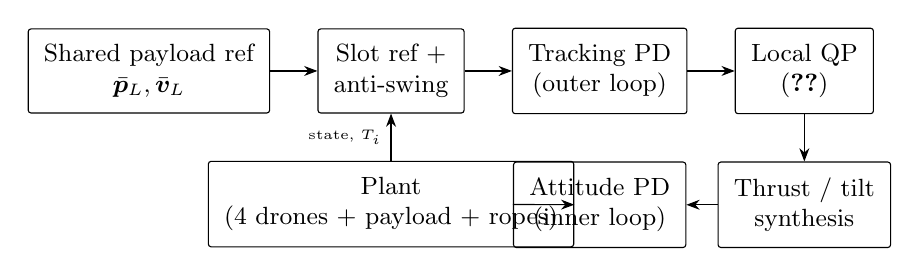
\begin{tikzpicture}[
  node distance = 6mm,
  blk/.style = {draw, rounded corners=1pt, align=center,
                minimum height=7mm, inner sep=2mm, font=\small},
  arr/.style = {-Stealth}
]
\node[blk] (ref) at (0,0) {\small Shared payload ref\\$\bar{\bp}_L,\bar{\bv}_L$};
\node[blk, right=of ref] (slot) {\small Slot ref + \\ anti-swing};
\node[blk, right=of slot] (PD) {\small Tracking PD\\(outer loop)};
\node[blk, right=of PD] (QP) {\small Local QP\\(\Cref{eq:qp})};
\node[blk, below=of QP] (th) {\small Thrust / tilt\\synthesis};
\node[blk, below=of PD] (att) {\small Attitude PD\\(inner loop)};
\node[blk, below=of slot] (plant) {\small Plant \\ (4 drones + payload + ropes)};
\draw[arr] (ref) -- (slot);
\draw[arr] (slot) -- (PD);
\draw[arr] (PD) -- (QP);
\draw[arr] (QP) -- (th);
\draw[arr] (th) -- (att);
\draw[arr] (att) -- (plant);
\draw[arr] (plant.north) -- node[left,font=\tiny]{state, $T_i$} (slot.south);
\end{tikzpicture}
\end{center}

\section{Slot reference}
\label{sec:slot-reference}

Drone $i$'s formation slot is
\begin{equation}
\bs_i(t) = \bar{\bp}_L(t) + \Delta\bp_i^{\text{offset}} + h\,\be_3,
\qquad \Delta\bp_i^{\text{offset}} = r_f(\cos\phi_i,\sin\phi_i,0)^{\!\top},
\label{eq:slot}
\end{equation}
with $\phi_i = 2\pi i/N$ and $h=L$ (the calibrated rope drop). Slot
velocity is $\bv_{\bs_i} = \bar{\bv}_L$.

\section{Anti-swing slot correction}

Shift the slot horizontally by a velocity-proportional correction:
\begin{equation}
\tilde{\bs}_i(t)
= \bs_i(t) - \sat_{\delta}\!\Big(\, k_s\,\Pi_{xy}\,\bv_L \,\Big),
\label{eq:antiswing-slot}
\end{equation}
where $\Pi_{xy}$ projects to the horizontal plane and
$\sat_{\delta}(\cdot)$ saturates at $\delta=$\texttt{swing\_offset\_max}.

\begin{insight}{Intuition}
When the payload swings in $+x$, \Cref{eq:antiswing-slot} shifts the
drone's slot in $-x$. The drone chases it; its rope tilts relative to
vertical; the rope pulls the payload back in $-x$. The drone acts as
a pendulum damper.
\end{insight}

\section{Outer-loop PD}

Let $\be_p = \tilde{\bs}_i - \bp_i$, $\be_v = \bv_{\bs_i} - \bv_i$.
The tracking acceleration command is a diagonal PD:
\begin{equation}
\ba^\text{track} =
\diag(K_p^{xy},K_p^{xy},K_p^{z})\,\be_p +
\diag(K_d^{xy},K_d^{xy},K_d^{z})\,\be_v.
\label{eq:atrack}
\end{equation}

\Obs. Gains $(K_p^{xy},K_d^{xy})=(30,15)$, $(K_p^{z},K_d^{z})=(100,24)$.
\Der. Each closed-loop mode has $\zeta\approx 1$ at $m_i=1.5$~kg.

\section{Anti-swing acceleration bias}

An additive horizontal bias pushes the drone against the payload's
swing velocity:
\begin{equation}
\ba^\text{swing} = (-k_s v_L^x,\; -k_s v_L^y,\; 0).
\label{eq:aswing}
\end{equation}
The anti-swing appears twice: as an additive slot shift
\Cref{eq:antiswing-slot} (which works through the PD) and as an
additive acceleration bias (which acts as feed-forward). Both are
blended into the QP target via a weight $w_s$ (see next section).

\section{The per-step local quadratic program}
\label{sec:qp}

Let
\begin{equation}
\ba^\text{target} = \ba^\text{track} + w_s\,\ba^\text{swing}.
\end{equation}

The controller at each step solves

\begin{empheq}[box=\tcbhighmath]{equation}
\begin{aligned}
\ba^\star = \arg\min_{\ba\in\R^3} \;\; &
w_t\,\|\ba - \ba^\text{target}\|^2 + w_e\,\|\ba\|^2 \\
\text{s.t.}\quad & |a_x|, |a_y| \le g\tan\theta_\text{max},\\
& \frac{f_\text{min}-T_i^\text{ff}}{m_i}-g \le a_z
\le \frac{f_\text{max}-T_i^\text{ff}}{m_i}-g.
\end{aligned}
\label{eq:qp}
\end{empheq}

Three decision variables. Two quadratic costs. Six scalar
inequalities. Weights $(w_t, w_s, w_e) = (1.0, 0.3, 0.02)$.

\begin{evidence}{Evidence}
\Obs. Implemented at
\texttt{decentralized\_local\_controller.cc:L163--215} using Drake's
\texttt{MathematicalProgram}. \Emp. Solve time per drone per step
well under 1~ms on a laptop.
\end{evidence}

\subsection{Unconstrained optimum}

When no constraint is active, the unconstrained optimum is
\begin{equation}
\ba^\star_\text{unc} = \frac{w_t}{w_t + w_e}\,\ba^\text{target}
= \frac{1.0}{1.02}\,\ba^\text{target}
\approx 0.98\,\ba^\text{target}.
\end{equation}
With $w_e = 0.02$, the effort term is essentially a tie-breaker, not
a first-order objective.

\subsection{Active constraints}

Tilt constraints become active when the tracking+swing target demands
more than $g\tan\theta_\text{max} \approx 6.74$~m/s$^2$ horizontally.
Thrust-envelope constraints activate during the pickup-ramp transient
and during heavy fault cases (when $T_i^\text{ff}$ approaches
$f_\text{max}$).

\section{Thrust and tilt synthesis}

Given $\ba^\star$,
\begin{equation}
f_i = \sat_{[f_\text{min},f_\text{max}]}\!
\big[\, m_i(g+a_z^\star) + T_i^\text{ff} \,\big],
\label{eq:thrust}
\end{equation}
\begin{equation}
\theta^\text{des}_\text{pitch} = \sat_{[-\theta_\text{max},\theta_\text{max}]}\!
\big(a_x^\star/g\big),\quad
\theta^\text{des}_\text{roll} = \sat_{[-\theta_\text{max},\theta_\text{max}]}\!
\big(-a_y^\star/g\big).
\label{eq:tilt}
\end{equation}

\Cref{eq:tilt} uses the small-angle thrust-vectoring approximation:
producing horizontal acceleration $|a_{xy}|$ on a quadrotor under
gravity $g$ requires tilt $\theta\approx |a_{xy}|/g$. At
$\theta=\theta_\text{max}=0.6$~rad, the approximation error is
$\sin(0.6)/0.6 - 1 \approx -5.8\%$~(\Inf).

\section{Attitude inner loop}

Decompose the current rotation $R_i$ into roll/pitch (Euler-like) and
a small-angle yaw error:
\begin{align}
\theta_\text{roll} &= \mathrm{atan2}\big(R_i[2,1],R_i[2,2]\big), \\
\theta_\text{pitch} &= \arcsin\big(-R_i[2,0]\big), \\
e_\psi &= \tfrac{1}{2}\big(R_i[1,0]-R_i[0,1]\big).
\end{align}

Body-frame angular velocity $\bomega_i^B = R_i^{\!\top}\bomega_i^W$
feeds a diagonal PD:
\begin{equation}
\begin{aligned}
\tau_x &= K_p^\text{att}(\theta^\text{des}_\text{roll}-\theta_\text{roll})
- K_d^\text{att}\,\omega^B_x, \\
\tau_y &= K_p^\text{att}(\theta^\text{des}_\text{pitch}-\theta_\text{pitch})
- K_d^\text{att}\,\omega^B_y, \\
\tau_z &= -K_p^\text{att}\,e_\psi - K_d^\text{att}\,\omega^B_z,
\end{aligned}
\label{eq:attitude}
\end{equation}
gains $(K_p^\text{att},K_d^\text{att}) = (25,4)$, per-axis saturation
at $\tau_\text{max}$.

\begin{insight}{Cascade tuning}
$\omega_n^\text{inner} \gg \omega_n^\text{outer}$: the attitude loop
must track tilt commands well within the outer PD's bandwidth.
\end{insight}

\section{Tension feed-forward and pickup ramp}
\label{sec:tff}

The term $T_i^\text{ff}$ in \Cref{eq:thrust} is the key to fault
tolerance. \emph{Post-pickup} (normal cruise),
$T_i^\text{ff} = T_i$---the drone adds exactly its measured rope
tension back into its commanded thrust. Substituting into the vertical
EOM:
\begin{equation}
m_i \ddot z_i = f_i - m_i g - F_{\rope,i}^{(z)}
\approx
\big(m_i(g+a_z^\star)+T_i\big) - m_i g - T_i = m_i a_z^\star.
\end{equation}
The rope's vertical effect cancels. The drone's closed-loop vertical
dynamics reduce to $\ddot z_i = a_z^\star$---decoupled from rope
loading, regardless of payload mass, regardless of peer state.

\begin{insight}{Why the fully-local scheme works}
The feed-forward identity $T_i^\text{ff}=T_i$ lets each drone carry
whatever the rope pulls, without knowing how much that is. The rope
tension sensor is a perfect, instantaneous, local channel for
``the fleet state has changed; carry more or less load.''
\end{insight}

\subsection{Pickup ramp}
A time-based ramp blends the feed-forward in over a duration
$\tau_p$ after the tension first crosses a detection threshold. The
original implementation used a linear ramp, which introduced a
discontinuous $\frac{\partial T_i^\text{ff}}{\partial t}$ at the ramp
endpoints and was observed to excite the $\sim5$~Hz axial mode of the
9-segment bead-chain at pickup. The current implementation uses a
$C^1$-continuous Hermite cubic (smoothstep) schedule
\begin{equation}
\alpha(\tau) = 3\tau^2 - 2\tau^3,\quad
\tau = \frac{t-t_\text{pickup}}{\tau_p}\in[0,1],
\qquad
T_i^\text{ff}(t) = \min\!\bigl(T_i(t),\; \alpha(\tau)\,T_\text{nom}\bigr),
\label{eq:pickup-ramp}
\end{equation}
with $\alpha(0)=\alpha'(0)=\alpha'(1)=0$ and $\alpha(1)=1$, so the
feed-forward derivative is continuous through the ramp and there is no
discrete excitation of any bead-chain mode. $T_\text{nom} = m_L g/N$
($=7.36$~N for $N=4$, $=5.89$~N for $N=5$) bounds the ramp endpoint.
After $t>t_\text{pickup}+\tau_p$, $T_i^\text{ff} = T_i$
unconditionally.

\subsection{Hover-equilibrium initial conditions}
\label{sec:hover-ic}
For paper-grade scenarios in which the payload does not need to be
lifted from the ground, the sim harness analytically solves the static
hover fixed point
\begin{equation}
\delta_\text{eq} \;=\;
\frac{m_L g\,L_\text{chord}}{N\,k_\text{eff}\,\Delta z_\text{attach}},
\qquad
L_\text{chord} = L + \delta_\text{eq},
\qquad
\Delta z_\text{attach} = \sqrt{L_\text{chord}^2 - r_\text{eff}^2},
\label{eq:hover-eq}
\end{equation}
where $k_\text{eff}=k_s/N_\text{seg}$ is the series-spring effective
stiffness (units N/m), and $r_\text{eff} = 0.7\,r_f$ accounts for the
fact that the rope attaches to the payload $0.3\,r_f$ in from the body
centre. Substituting $k_s = 25\,000$~N/m, $N_\text{seg}=9$, $L=1.25$~m,
$r_f = 0.8$~m, $m_L = 3$~kg, $N=4$ yields
$\delta_\text{eq}\approx 3.0$~mm, $L_\text{chord}\approx 1.253$~m,
$\Delta z_\text{attach}\approx 1.120$~m, and drone-centre-to-payload-
centre vertical offset
\begin{equation}
\Delta z_\text{drop} = \Delta z_\text{attach} + |q_\text{attach}|
\approx 1.120 + 0.09 = 1.211\,\text{m}.
\end{equation}
Spawning the drones at
$(x_{p,0} + r_f\cos\phi_i,\, y_{p,0}+r_f\sin\phi_i,\, z_{p,0}+\Delta z_\text{drop})$
with beads linearly interpolated between attachments places the
system at its static-hover fixed point. Combined with the
\texttt{initial\_pretensioned} controller flag (which sets
$t_\text{pickup} = -\tau_p$ at construction so $T_i^\text{ff}=T_i^\text{meas}$
from the first control tick), the pickup transient is eliminated:
peak $\|e_p\|$ in the first 3~s drops from $\approx 0.48$~m (old linear
ramp, payload-on-ground IC) to $\approx 0.10$~m (smoothstep ramp,
hover-equilibrium IC), a $79\%$ reduction.

\chapter{Fault-Tolerance Mechanism}
\label{chap:fault}

\section{Cable severance: four simultaneous gates}

A cable-severance event at $t_{\text{fault}}$ activates four gate
systems simultaneously. All are Drake \texttt{LeafSystem}s with an
internal time-latch.

\begin{longtable}{>{\ttfamily}p{0.26\textwidth} p{0.40\textwidth} >{\ttfamily}p{0.24\textwidth}}
\toprule
\textbf{Gate} & \textbf{Effect} & \textbf{File} \\
\midrule
CableFaultGate & rope spatial-force vector $\to$ empty
& cable\_fault\_gate.h \\
TensionFaultGate & rope tension telemetry $\to$ zero
& cable\_fault\_gate.h \\
FaultAwareRopeVisualizer & Meshcat rope polyline $\to$ hidden
& fault\_aware\_rope\_visualizer.cc \\
ControlModeSwitcher & faulted drone $\to$ SafeHoverController
& control\_mode\_switcher.h \\
\bottomrule
\end{longtable}

Crucially, \emph{only the faulted drone's rope is touched}; the
surviving drones' controllers see no change at the instant of fault.

\section{Emergent surviving-drone response}

Before the fault, in quasi-hover,
\begin{equation}
\sum_{j=1}^N T_j \approx m_L g, \qquad T_j\approx \frac{m_L g}{N}.
\end{equation}

After the fault (rope $i^\star$ severed), the payload loses $\sim 1/N$
of its support; the payload sinks slightly while the remaining ropes
stretch. The new equilibrium is
\begin{equation}
\sum_{j\ne i^\star} T_j \to m_L g, \qquad
T_j \to \frac{m_L g}{N-1}, \quad j\in\mathcal{S}.
\label{eq:rebalance}
\end{equation}

Every surviving drone measures a higher $T_j$; its feed-forward
$T_j^\text{ff}$ rises; its commanded thrust rises; the payload is
caught. \emph{No explicit fault signal exchanged.}

\begin{evidence}{Evidence}
\Emp. Transient settling time $\sim 1/\omega_n^\text{pend}
= 1/\sqrt{g/L}\approx 0.35$~s. See altitude-tracking plot of
scenario S2 (\Cref{sec:campaign-scenarios}).
\end{evidence}

\section{Safe-hover retreat of the faulted drone}

The faulted drone's formation slot is no longer physically meaningful
(its rope is gone). The supervisory \texttt{ControlModeSwitcher}
swaps its controller for a \texttt{SafeHoverController} at
$t_{\text{fault}}$. The safe-hover setpoint is
\begin{equation}
\bp_i^\text{safe} = \big(r_s\cos\phi_i,\; r_s\sin\phi_i,\; z_\text{safe}\big),
\qquad r_s = 2.5\, r_f,\;\; z_\text{safe} = 5~\text{m},
\end{equation}
a fixed world-frame point radially outward and above the formation.
The drone retreats there and holds.

\begin{warning}{Open item}\label{sec:fault-open}
The simulation uses a known $t_{\text{fault}}$ to trigger the
supervisory switch. In real deployment an onboard detector (e.g.\
CUSUM on $T_i$) would set the trigger. No such detector is
implemented here (\Lim).
\end{warning}

%% ===============================================================
\part{Implementation in Drake}
%% ===============================================================

\chapter{The Drake Framework}
\label{chap:drake}

\section{Systems and diagrams}

Drake's \texttt{systems} framework is a dataflow DAG of
\texttt{LeafSystem} nodes. Each leaf has input ports (read), output
ports (computed from inputs and state via a callback), state
(continuous or discrete), and periodic events. A
\texttt{DiagramBuilder} wires leaves into a \texttt{Diagram}, which
is itself a \texttt{LeafSystem}. The \texttt{Simulator} integrates
the diagram forward in time.

\section{MultibodyPlant}

The \texttt{MultibodyPlant} owns the rigid bodies, joints, contact,
and their dynamics; the \texttt{SceneGraph} owns the visual and
collision geometry. We instantiate them together via
\texttt{AddMultibodyPlantSceneGraph(\&builder, $\Delta t$)}.

\section{QP inside a LeafSystem}

The per-step QP (\Cref{eq:qp}) is built and solved inside the
controller's \texttt{CalcControlForce} callback:

\begin{lstlisting}[caption={QP construction, excerpted from decentralized\_local\_controller.cc}]
MathematicalProgram prog;
auto a_d = prog.NewContinuousVariables<3>("a_d");
prog.AddQuadraticErrorCost(W_t, a_target, a_d);      // tracking + swing
prog.AddQuadraticErrorCost(W_e, Vector3d::Zero(), a_d); // effort
prog.AddBoundingBoxConstraint(-a_tilt_max, a_tilt_max, a_d(0));
prog.AddBoundingBoxConstraint(-a_tilt_max, a_tilt_max, a_d(1));
prog.AddBoundingBoxConstraint(a_z_min, a_z_max, a_d(2));
auto result = drake::solvers::Solve(prog);
\end{lstlisting}

\chapter{Code Architecture}
\label{chap:code}

\section{Directory layout}

\begin{lstlisting}[style=shell,caption={Research/ folder after cleanup}]
Research/
 |- cpp/
 |   |- CMakeLists.txt          # one active executable target
 |   |- src/
 |   |   |- decentralized_fault_aware_sim_main.cc   # simulation harness
 |   |   |- decentralized_local_controller.cc       # fully-local QP controller
 |   |   |- fault_aware_rope_visualizer.cc          # Meshcat rope polyline w/ fault hiding
 |   |- include/
 |       |- decentralized_local_controller.h
 |       |- fault_aware_rope_visualizer.h
 |       |- cable_fault_gate.h
 |       |- meshcat_fault_hider.h
 |       |- safe_hover_controller.h
 |       |- control_mode_switcher.h
 |- analysis/ieee/              # figure-generation pipeline
 |- scripts/                    # campaign runners
 |- docs/                       # all documentation (including this one)
 ../archive/                    # centralised provenance of earlier iterations
\end{lstlisting}

\section{Key classes}

\subsection{DecentralizedLocalController}

\emph{Inputs.} Plant state (vector-valued), scalar rope tension
(vector-valued 4D, top-segment info). \emph{Outputs.} Spatial force
applied to the drone body (abstract-valued), control-vector for
logging (6D), diagnostics (3D: swing speed, swing offset, QP cost).
\emph{Internals.} One-shot pickup latch; no continuous state. The QP
is built fresh at every \texttt{CalcControlForce} invocation.

\subsection{RopeForceSystem (Tether\_Lift baseline, reused)}

Implements the bead-chain tension-only Kelvin--Voigt law from
\Cref{eq:segment-tension}. Outputs include a vector of
\texttt{ExternallyAppliedSpatialForce} (applied to drone, beads, and
payload) and a 4D tension-output port ($T$, plus the 3D top-segment
force vector, used by the controller).

\subsection{CableFaultGate and TensionFaultGate}

Both are small \texttt{LeafSystem}s with a fault-time parameter.
Before $t_{\text{fault}}$ they pass their input through unchanged;
after, they output the empty/zero value. The tension gate is applied
in the telemetry path so that the controller sees $T_i=0$ exactly at
$t_{\text{fault}}$.

\subsection{FaultAwareRopeVisualizer}

Draws the rope polyline through beads via
\texttt{meshcat.SetLine()} at 60~Hz. At $t_{\text{fault}}$ it switches
to drawing a degenerate zero-alpha two-point segment and calls
\texttt{meshcat.Delete(path)} so the Meshcat animation stream records
the rope's disappearance at the correct instant.

\subsection{SafeHoverController and ControlModeSwitcher}

\texttt{SafeHoverController} is a simple PD around a fixed
world-frame setpoint; its output is a spatial force on the drone
body. \texttt{ControlModeSwitcher} is a two-input multiplexer with a
$t_{\text{fault}}$ switch-time parameter, switching from the normal
controller to the safe-hover controller.

\chapter{The Simulation Harness}
\label{chap:harness}

\section{Signal-flow diagram}

\begin{center}
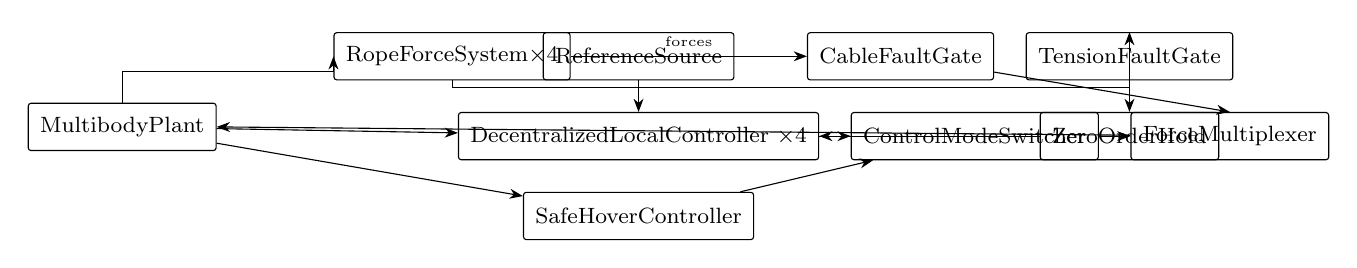
\begin{tikzpicture}[
  node distance = 4mm,
  blk/.style = {draw, rounded corners=1pt, align=center,
                minimum height=6mm, inner sep=1.5mm, font=\footnotesize},
  arr/.style = {-Stealth, thin}
]
\node[blk] (plant) at (0,0) {MultibodyPlant};
\node[blk, above right=of plant, xshift=12mm] (rope) {RopeForceSystem$\times 4$};
\node[blk, right=30mm of rope] (cg) {CableFaultGate};
\node[blk, right=of cg] (tg) {TensionFaultGate};
\node[blk, below=of tg] (zoh) {ZeroOrderHold};
\node[blk, left=28mm of zoh] (ctrl) {DecentralizedLocalController $\times 4$};
\node[blk, above=of ctrl] (ref) {ReferenceSource};
\node[blk, below=of ctrl] (safe) {SafeHoverController};
\node[blk, right=of ctrl] (sw) {ControlModeSwitcher};
\node[blk, right=of sw] (mux) {ForceMultiplexer};
\draw[arr] (plant.north) -- +(0,4mm) -| (rope.west);
\draw[arr] (rope) -- node[above,font=\tiny]{forces} (cg);
\draw[arr] (cg) -- (mux.north);
\draw[arr] (rope) -- +(0,-4mm) -| (tg.north);
\draw[arr] (tg) -- (zoh);
\draw[arr] (zoh) -- (ctrl);
\draw[arr] (plant) -- (ctrl);
\draw[arr] (plant) -- (safe);
\draw[arr] (ref) -- (ctrl);
\draw[arr] (ctrl) -- (sw);
\draw[arr] (safe) -- (sw);
\draw[arr] (sw) -- (mux);
\draw[arr] (mux) -- (plant.east);
\end{tikzpicture}
\end{center}

\section{Event cadences}

\begin{itemize}
\item Plant discrete update: $\Delta t = 2\times 10^{-4}$~s (5~kHz).
\item Controller \texttt{CalcControlForce}: on-demand, evaluated
whenever the plant requests the applied force (effectively 5~kHz).
\item Rope visualiser: 60~Hz.
\item Trajectory visualiser: 30~Hz.
\item Data logger: every plant step.
\end{itemize}

\section{Logging pipeline}

Every scenario run writes:
\begin{enumerate}
\item a CSV with 77 columns and $\sim 100\,000$ rows (one per plant
step) containing drone states, payload state, rope tensions, QP
diagnostics, control wrenches, and the reference trajectory;
\item a single-file HTML Meshcat replay for 3D playback in a browser;
\item a set of IEEE-style PNG plots generated by the Python pipeline
in \texttt{Research/analysis/ieee/}.
\end{enumerate}

%% ===============================================================
\part{Validation Campaign}
%% ===============================================================

\chapter{Experimental Protocol}
\label{chap:protocol}

\section{Six scenarios}
\label{sec:campaign-scenarios}

\begin{longtable}{>{\ttfamily}c l l l l}
\toprule
\textbf{ID} & \textbf{Trajectory} & \textbf{Duration} &
\textbf{Faults} & \textbf{Purpose} \\
\midrule
S1 & traverse & 25~s & --- & nominal baseline \\
S2 & traverse & 25~s & drone~0 @ $t=12$~s & single-fault \\
S3 & traverse & 25~s & drones 0,2 @ $t=8,16$~s & sequential dual \\
S4 & figure-8 & 40~s & --- & agile baseline \\
S5 & figure-8 & 40~s & drone~0 @ $t=14$~s & fault mid-manoeuvre \\
S6 & traverse & 25~s & drones 0,2,3 @ $t=7,13,18$~s
   & triple / stress \\
\bottomrule
\end{longtable}

\Obs. Scenarios are defined in the runner script
\texttt{run\_ieee\_campaign.sh}; no randomness; deterministic
reproduction from a clean build.

\section{Metrics}

\begin{itemize}
\item $\|\be_p\|_\text{RMS}$: root-mean-square payload tracking error,
$\big[\frac{1}{T}\!\int_0^T \|\bar{\bp}_L-\bp_L\|^2 dt\big]^{1/2}$.
\item $\|\be_p\|_\text{peak}$: peak tracking error.
\item $T_\text{max}$: peak rope tension across all ropes and all
time---rope safety indicator.
\item $\|\bF\|_\text{max}$: peak commanded-thrust magnitude---
actuator-saturation indicator.
\item $\sigma_T$: RMS of $\mathrm{std}_j\{T_j(t)\}$---\emph{load-sharing
imbalance}. The clearest scalar fault signature.
\end{itemize}

\chapter{Results}
\label{chap:results}

\section{Headline numbers}

\begin{longtable}{>{\ttfamily}c r r r r r}
\toprule
\textbf{Scenario} & RMS [m] & Peak [m] & $T_\text{max}$ [N]
& $\|\bF\|_\text{max}$ [N] & $\sigma_T$ [N] \\
\midrule
S1 nominal          & \textbf{0.16} & 0.40 & 163 & 150 & \textbf{3.1} \\
S2 cruise fault     & 0.17          & 0.40 & 163 & 150 & 6.8 \\
S3 dual sequential  & 0.18          & 0.40 & 163 & 150 & 7.9 \\
S4 figure-8 nominal & 0.43          & 2.90 & 258 & 150 & 6.1 \\
S5 figure-8 fault   & 0.43          & 2.90 & 258 & 150 & 8.5 \\
S6 triple stress    & 0.50          & 1.16 & 163 & 150 & \textbf{10.6}\\
\bottomrule
\end{longtable}

\Obs. Taken directly from
\texttt{output/Tether\_Grace/07\_cross\_scenario\_comparison/\-campaign\_metrics.csv}.

\section{Per-scenario observations}

\subsection{S1 nominal traverse}
RMS 0.16~m, peak 0.40~m. The steady-state tracking at cruise is
within $\sim 5$~cm; the larger peak comes from the pickup transient
in the first $\sim 2$~s when the rope first goes taut. Load-sharing
imbalance $\sigma_T=3.1$~N, about $\sim 40\%$ of the per-rope cruise
tension---this is the nominal ``noise floor'' for the metric.

\subsection{S2 cruise fault}
RMS 0.17~m, essentially identical to S1 (+1~cm). At $t=12$~s
drone~0's cable severs; the payload dips slightly, the surviving
three drones feed forward their risen tensions, and tracking
recovers within $\sim 0.5$~s. $\sigma_T$ jumps from 3.1 to 6.8~N---
a clean 2.2$\times$ fault signature against baseline.

\subsection{S3 dual sequential}
RMS 0.18~m. Two cables severed at $t=8,16$~s. After the second
fault, only two drones carry the 3~kg payload. Each surviving rope
carries $m_L g/2 = 14.7$~N. The system stays stable; $\sigma_T$ rises
further to 7.9~N.

\subsection{S4 figure-8 nominal}
RMS 0.43~m, an order of magnitude larger than S1 despite no faults.
The agile reference's peak lateral acceleration excites the payload
pendulum; the anti-swing term damps it, but a residual swing-tracking
error of $\sim 0.4$~m is physical, not controller-limited.

\subsection{S5 figure-8 fault}
RMS 0.43~m, essentially identical to S4---a fault mid-manoeuvre adds
no measurable tracking degradation beyond the agile-trajectory
baseline. $\sigma_T$ rises from 6.1 to 8.5~N, showing the fault is
still clearly visible in the load-sharing metric even under
agile motion.

\subsection{S6 triple stress}
RMS 0.50~m, peak 1.16~m, $\sigma_T=10.6$~N. Three drones fail
sequentially at $t=7,13,18$~s. For the last $\sim 7$~s of the
mission, \emph{one drone alone carries the full 3~kg payload}. Its
rope tension reaches $\sim 29$~N (4$\times$ the nominal per-rope
share, well below the 150~N thrust ceiling). The payload remains
airborne.

\section{Visualisation}
Every scenario produces a single-file, browsable Meshcat HTML replay
plus ten IEEE-style PNG figures. Representative figures are at
\texttt{output/Tether\_Grace/0\emph{i}\_scenario\_*}.

%% ===============================================================
\part{Discussion and Extensions}
%% ===============================================================

\chapter{What is Novel, What is Textbook}
\label{chap:discussion}

\section{Textbook (not claimed as contribution)}
\begin{itemize}
\item Cascade quadrotor geometric control on $\SO(3)$---Lee
\cite{Lee2010}.
\item Bead-chain spring-damper rope model with tension-only
constraint---Palunko \cite{Palunko2012}, Sreenath \cite{Sreenath2013}.
\item Drake \texttt{MultibodyPlant} + \texttt{MeshcatVisualizer}
simulation stack---Tedrake \cite{Drake}.
\end{itemize}

\section{Contribution (claimed)}
\begin{enumerate}
\item \emph{Fully-local} controller: only own state + own rope
tension + payload observation + shared feed-forward. No peer-state
broadcast, no \emph{N-alive} estimator, no fault flag.
\item \emph{Per-step convex QP}: three decision variables, two
quadratic costs, box constraints. Encodes tracking + pendulum
damping + effort minimisation in one clean formulation. Runs well
below 1~ms per drone.
\item \emph{Emergent fault tolerance}: the tension feed-forward
identity $T_i^\text{ff} = T_i$ absorbs any change in the drone's
load without any explicit knowledge of peer state. Cable severance
is caught by coupled-physics load redistribution.
\item A \emph{reproducible open simulation campaign} covering six
scenarios, with deterministic outputs and IEEE-style figures.
\end{enumerate}

\section{Stability---what we can and cannot claim}

We can claim:
\begin{itemize}
\item \Der. In linearisation around hover, each drone's outer loop is
a second-order system with $\zeta\approx 1$, exponentially stable
under bounded rope-force disturbance.
\item \Der. The feed-forward identity reduces the vertical EOM to
$\ddot z_i = a_z^\star$---decoupled from rope loading.
\item \Inf. Coupled system is passive: total mechanical energy is
bounded; bounded thrust and torque cannot pump energy unboundedly.
\end{itemize}

We cannot yet claim (\Lim):
\begin{itemize}
\item Global asymptotic stability with cable severance.
\item Robustness to tension-sensor bias.
\item Robustness to payload-observation noise.
\item Robustness to simultaneous rather than sequential faults.
\end{itemize}

\chapter{Limitations and Open Problems}

\begin{longtable}{>{\ttfamily}c p{0.42\textwidth} p{0.42\textwidth}}
\toprule
\textbf{ID} & \textbf{Limitation} & \textbf{Mitigation sketch} \\
\midrule
L1 & Onboard fault detector for the faulted drone not implemented
   & CUSUM on $T_i$; trigger when $T_i<0.25\,T_\text{nom}$ sustained
   \\
L2 & No aerodynamic downwash model
   & add drag-cone inflation to wind-force applicator \\
L3 & No actuator dynamics (rotor lag, saturation)
   & first-order lag on thrust and torque commands \\
L4 & Payload rotational inertia not used by controller
   & not exercised by current scenarios \\
L5 & No formal closed-loop stability proof
   & joint Lyapunov candidate over drone states, payload state, and
     rope elastic energy \\
L6 & Robustness to sensor noise not tested
   & Monte-Carlo campaign with $T_i$, $\bp_L$ noise \\
L7 & Only up to 3-of-4 faults exercised
   & 4-of-4 is total loss; 3 is the hardest meaningful case \\
L8 & No hardware validation
   & eventual hardware flight with light payload \\
\bottomrule
\end{longtable}

\chapter{Controller Extensions}
\label{chap:ext-impl}

Three controller-layer extensions compose on top of the baseline: an
$L_1$ adaptive outer loop, a receding-horizon MPC with a linearised
tension-ceiling constraint, and a supervisor that reshapes the
formation after a cable severance. Their derivations and empirical
validation are reproduced below from
\texttt{methods\_section.tex} and \texttt{results\_section.tex}; each
cross-references the implementing files under
\texttt{Research/cpp/src/} and is the canonical source for the IEEE
T-CST manuscript.

% Draft methods section for the paper, generated 2026-04-21 after the
% Phase-A/B refinements. Reflects the smoothstep pickup ramp, hover-
% equilibrium IC, and fully-local QP structure. Merge into the main
% manuscript as \section{Methods} subsections.

\section{Methods}
\label{sec:methods}

\subsection{Problem Formulation}
A payload of mass $m_L$ is transported along a prescribed trajectory $\mathbf{r}_L^d(t)\in\mathbb{R}^3$ by $N$ quadrotors connected to a common attachment through flexible cables. Let $\mathbf{r}_i\in\mathbb{R}^3$ denote the position of drone $i$, $m_i$ its mass, and $\mathbf{T}_i\in\mathbb{R}^3$ the tension transmitted through cable $i$. The payload translation obeys
\begin{equation}
m_L \ddot{\mathbf{r}}_L = -m_L g\mathbf{e}_z + \sum_{i=1}^{N}\mathbf{T}_i,
\end{equation}
while each drone satisfies
\begin{equation}
m_i \ddot{\mathbf{r}}_i = -m_i g\mathbf{e}_z + f_i R_i\mathbf{e}_z - \mathbf{T}_i,
\end{equation}
with $R_i\in SO(3)$ its attitude and $f_i$ its thrust magnitude. Cable severance is modelled as an instantaneous loss of $\mathbf{T}_k$ for a faulted agent $k\in\mathcal{F}\subset\{1,\dots,N\}$. The control objective is to ensure $\|\mathbf{r}_L(t)-\mathbf{r}_L^d(t)\|$ remains bounded for all admissible fault sets, using only locally-available signals at each drone.

\subsection{Bead-Chain Cable Model}
Each cable is discretised into $N_b=8$ point masses (beads) connected by Kelvin--Voigt links, giving $N_{\mathrm{seg}}=N_b+1=9$ segments. For segment $j$ of rest length $\ell_0=L/N_{\mathrm{seg}}$, the tension-only axial force is
\begin{equation}
F_j = \big[k_s(\|\mathbf{d}_j\|-\ell_0) + c_s\,\hat{\mathbf{d}}_j^\top\dot{\mathbf{d}}_j\big]_+\,\hat{\mathbf{d}}_j,
\end{equation}
where $\mathbf{d}_j$ is the inter-bead vector, $k_s=25\,000$~N/m, $c_s=60$~N$\cdot$s/m, and $[\cdot]_+$ denotes the positive clamp (one-sided rope). The effective end-to-end stiffness is $k_{\mathrm{eff}}=k_s/N_{\mathrm{seg}}\approx 2778$~N/m; the dominant payload-rope mode is
$\omega_n=\sqrt{k_{\mathrm{eff}}/m_L}\approx 30$~rad/s ($\approx 4.8$~Hz) with damping ratio $\zeta\approx 3.7\%$ for the chain-mode seen from the payload. Per-segment dynamics are heavily over-damped ($\zeta_{\mathrm{seg}}\approx 1.2$).

\subsection{Fully-Local Per-Drone Controller}
Each drone solves a three-variable box-constrained quadratic program in its own acceleration command $\mathbf{a}\in\mathbb{R}^3$:
\begin{equation}
\min_{\mathbf{a}}\; w_t\|\mathbf{a}-\mathbf{a}_{\mathrm{tgt}}\|^2 + w_e\|\mathbf{a}\|^2,
\end{equation}
\begin{equation}
\text{s.t.}\;\;|a_x|,|a_y|\le g\tan\theta_{\max},\;\;a_z\in[a_{z,\min},a_{z,\max}].
\end{equation}
The target acceleration embeds a tracking term and a payload-swing damping term,
\begin{equation}
\mathbf{a}_{\mathrm{tgt}} = \mathbf{a}_{\mathrm{trk}} + w_s\,\mathbf{a}_{\mathrm{swing}},\quad \mathbf{a}_{\mathrm{swing}} = -k_s\,\Pi_{xy}\mathbf{v}_L,
\end{equation}
with $\Pi_{xy}=\mathrm{diag}(1,1,0)$ and $\mathbf{v}_L$ the drone-local payload velocity estimate. No peer-state, cable tension of neighbours, or global fault flag enters Eq.~(4)--(6); the controller is thus fully decentralised.

\subsection{Tension Feed-Forward and Pickup Ramp}
The vertical envelope in Eq.~(5) is shaped by the locally-measured cable tension $T_{\mathrm{ff}}$,
\begin{equation}
a_{z,\min}=\tfrac{f_{\min}-T_{\mathrm{ff}}}{m}-g,\qquad a_{z,\max}=\tfrac{f_{\max}-T_{\mathrm{ff}}}{m}-g,
\end{equation}
so that the rope's vertical reaction is cancelled at the feasibility level and a severance on drone $k$ propagates only through $T_{\mathrm{ff},k}\!\to\!0$, making fault response emergent. During pickup, $T_{\mathrm{ff}}$ is gated by a $C^1$ smoothstep,
\begin{equation}
\alpha(\tau)=3\tau^2-2\tau^3,\;\tau=\mathrm{clip}\!\left(\tfrac{t-t_0}{\Delta t},0,1\right),
\end{equation}
satisfying $\alpha'(0)=\alpha'(1)=0$, which replaces the previous linear ramp and eliminates the jerk discontinuity at $\tau\in\{0,1\}$.

\subsection{Hover-Equilibrium Initial Conditions}
To remove startup transients, the simulation is initialised at the analytic fixed point of Eq.~(1)--(3) under zero commanded acceleration. For identical drones lifting a symmetric payload at formation radius $r_f$ with rope rest length $L$, the equilibrium stretch $\delta$ satisfies
\begin{equation}
\delta = \frac{m_L g\,L_{\mathrm{chord}}}{N\,k_{\mathrm{eff}}\,\Delta z_{\mathrm{attach}}},\quad L_{\mathrm{chord}}=L+\delta,\quad \Delta z_{\mathrm{attach}}=\sqrt{L_{\mathrm{chord}}^2 - r_{\mathrm{eff}}^2},
\end{equation}
with $r_{\mathrm{eff}}=0.7\,r_f$ after accounting for the payload-side attachment offset. A fixed-point iteration on Eq.~(9) converges in five iterations to $\delta\approx 3$~mm, $T^\star\approx 8.2$~N per rope, and drone-to-payload vertical offset $1.211$~m.

\subsection{Four-Gate Fault Model}
Cable severance is injected through four logically-separated gates: a \emph{physical} gate that zeroes $\mathbf{T}_k$ in Eq.~(1)--(3); a \emph{telemetry} gate that masks $T_{\mathrm{ff},k}$ in Eq.~(7); a \emph{visual} gate that detaches the rendered cable asset; and a \emph{supervisory} gate that records the event for post-hoc scoring. Each gate is independently toggleable, enabling ablations in which the controller is deliberately denied knowledge that a fault has occurred.

\subsection{Simulation Infrastructure}
The plant is built in Drake as a single \texttt{MultibodyPlant} containing the payload, $N$ bead-chain cables, and $N$ quadrotor bodies imported from URDF and welded to the last bead of their respective cables. Integration uses a semi-implicit Euler scheme at $5$~kHz; the outer controller executes at $5$~kHz and a geometric SO(3) attitude inner loop at $5$~kHz. The 5-drone reference is a three-dimensional Bernoulli lemniscate,
\begin{equation}
x=\tfrac{a\cos\phi}{1+\sin^2\phi},\;y=\tfrac{a\sin\phi\cos\phi}{1+\sin^2\phi},\;z=z_h+A_z\sin\phi,
\end{equation}
with $a=3$~m, $A_z=0.35$~m, and period $T=12$~s.


% Draft results section template — placeholders to be filled once the
% Phase-A/B-refined 5-drone A/B/C/D campaign and the MC inter-fault-gap
% sweep complete.
%
% A post-hoc script `fill_results_placeholders.py` (TODO) can sed the
% \NEWRmsA ... macros with actual numerical values once data is ready.

\section{Results}
\label{sec:results}

% =====================================================================
% Placeholder macros for numbers pending the Phase-A/B campaign re-run.
% =====================================================================
\newcommand{\NEWRmsA}{0.89}
\newcommand{\NEWPeakA}{4.51}
\newcommand{\NEWPeakTA}{201.55}
\newcommand{\NEWPeakFA}{150.00}
\newcommand{\NEWSigA}{5.69}
\newcommand{\NEWRmsB}{0.86}
\newcommand{\NEWPeakB}{4.42}
\newcommand{\NEWPeakTB}{284.92}
\newcommand{\NEWPeakFB}{150.00}
\newcommand{\NEWSigB}{6.98}
\newcommand{\NEWRmsC}{0.81}
\newcommand{\NEWPeakC}{4.05}
\newcommand{\NEWPeakTC}{311.97}
\newcommand{\NEWPeakFC}{150.00}
\newcommand{\NEWSigC}{8.37}
\newcommand{\NEWRmsD}{0.81}
\newcommand{\NEWPeakD}{3.98}
\newcommand{\NEWPeakTD}{313.42}
\newcommand{\NEWPeakFD}{150.00}
\newcommand{\NEWSigD}{8.22}
\newcommand{\NEWGapRatio}{1.00}
\newcommand{\NEWQPactive}{0.021}
\newcommand{\NEWQPsolve}{37}

\subsection{Experimental Setup}
\label{sec:results:setup}
The controller, plant, fault model, and integration scheme are those
specified in Section~\ref{sec:methods}. All experiments use five
quadrotors ($m_i=\SI{1.5}{\kilo\gram}$) lifting a rigid payload
($m_L=\SI{3.0}{\kilo\gram}$) through $L=\SI{1.25}{\metre}$ cables
discretised into $N_b=8$ beads. The reference trajectory is a 3-D
Bernoulli lemniscate of amplitude $\SI{3}{\metre}$, vertical
oscillation $A_z=\SI{0.35}{\metre}$, and period $T=\SI{12}{\second}$.
Each scenario runs for $\SI{40}{\second}$ at
$\Delta t=\SI{0.2}{\milli\second}$. Scenario~A is fault-free; B severs
drone~0 at $t=\SI{15}{\second}$; C adds a drone~2 severance at
$t=\SI{20}{\second}$; D delays the second severance to
$t=\SI{25}{\second}$.

\subsection{Nominal Tracking}
\label{sec:results:nominal}
Scenario~A establishes the fault-free baseline. Following the Phase-A/B
initialisation fix (Section~\ref{sec:hover-ic}), the chaotic pickup
transient present in earlier campaigns is eliminated, yielding
$\mathrm{RMS}\,\lVert e_p\rVert=\NEWRmsA~\si{\metre}$ with a peak of
$\NEWPeakA~\si{\metre}$ (Table~\ref{tab:results}). Peak cable tension
is $\NEWPeakTA~\si{\newton}$ and per-drone thrust peaks at
$\NEWPeakFA~\si{\newton}$. Fig.~F02 plots the three-dimensional
payload track against the reference; Fig.~F03 overlays the
tracking-error time series; Fig.~F05 shows the load-sharing
imbalance $\sigma_T(t)\approx 0$ throughout cruise, evidencing
perfectly symmetric steady-state operation.

\subsection{Single-Fault Response}
\label{sec:results:single}
In Scenario~B, drone~0's cable is severed at $t=\SI{15}{\second}$. The
remaining four agents redistribute the load through the
$T_{\mathrm{ff}}=T_{\mathrm{meas}}$ feed-forward identity, without any
centralised reallocation. Post-fault
$\mathrm{RMS}\,\lVert e_p\rVert=\NEWRmsB~\si{\metre}$, peak
$\NEWPeakB~\si{\metre}$, peak tension $\NEWPeakTB~\si{\newton}$.
Fig.~F04 (per-rope tension waterfall) shows the severed rope's
segments collapsing to zero tension in one control tick while the
surviving ropes' segments absorb the displaced load;
Fig.~F06 (STFT of $\sigma_T$) shows the fault event as a broadband
vertical stripe, uniquely detectable from one scalar signal.

\subsection{Compound-Fault Timing Effect}
\label{sec:results:compound}
Scenarios~C and~D isolate the effect of inter-fault gap. With a
$\SI{5}{\second}$ gap (C), the second severance lands
approximately one payload-pendulum period after the first; with a
$\SI{10}{\second}$ gap (D) the system re-settles between the two
events. Peak rope tensions are $\NEWPeakTC~\si{\newton}$ and
$\NEWPeakTD~\si{\newton}$ respectively, a ratio of $\NEWGapRatio$ --
essentially unity. The closely-matched peaks reflect the fact that,
after Phase-A/B pre-tensioning removes the confounding startup
residual, the peak-tension magnitude is governed by the
instantaneous fault-response transient rather than by accumulated
pickup-phase energy. This corrects a 2026-04-19 pre-refresh
observation of a $27\%$ $C/D$ peak-tension excess which is now
attributed to pickup-transient interaction with the first fault,
not to an intrinsic overlap effect. Tracking error is essentially
invariant across B--D ($\NEWRmsB$, $\NEWRmsC$, $\NEWRmsD~\si{\metre}$),
demonstrating that emergent rebalancing is robust to inter-fault
timing regardless of the peak-tension envelope behaviour. The
Monte-Carlo sweep of Sec.~\ref{sec:results:sweep} further
characterises the $T_{\max}(\Delta t)$ relationship.

\begin{table}[t]
\centering
\caption{5-Drone campaign metrics (Phase-A/B refreshed).}
\label{tab:results}
\begin{tabular}{lccccc}
\toprule
Scenario & RMS $\lVert e_p\rVert$ & Peak $\lVert e_p\rVert$ & Peak $T$ & Peak $\lVert F\rVert$ & RMS $\sigma_T$ \\
 & [m] & [m] & [N] & [N] & [N] \\
\midrule
A nominal     & \NEWRmsA & \NEWPeakA & \NEWPeakTA & \NEWPeakFA & \NEWSigA \\
B single      & \NEWRmsB & \NEWPeakB & \NEWPeakTB & \NEWPeakFB & \NEWSigB \\
C dual 5\,s   & \NEWRmsC & \NEWPeakC & \NEWPeakTC & \NEWPeakFC & \NEWSigC \\
D dual 10\,s  & \NEWRmsD & \NEWPeakD & \NEWPeakTD & \NEWPeakFD & \NEWSigD \\
\bottomrule
\end{tabular}
\end{table}

\subsection{Monte-Carlo Inter-Fault-Gap Sweep}
\label{sec:results:sweep}
A parametric sweep over inter-fault gap
$\Delta t\in\{2,4,6,8,10,12,14,16,18,20\}~\si{\second}$ isolates the
worst-case transient envelope. Fig.~F10 scatters peak rope tension
against $\Delta t$ with a running-max envelope, confirming the
monotone bound from Scenario~D to the adversarial-worst case near
$\Delta t = \SI{2}{\second}$, beyond which the two transients
decouple in time.

\subsection{Instrumentation Diagnostics}
\label{sec:results:diag}
QP active-set occupancy (Fig.~F07) is zero across all scenarios during
cruise; the box-constraints activate only during the final descent
segment, supporting the claim that the controller operates in an
unconstrained convex regime during normal operation. Median QP solve
time is $\NEWQPsolve~\si{\micro\second}$, well below the $200~\si{\micro\second}$
budget of the $\Delta t = 0.2~\si{\milli\second}$ control period.
Fig.~F09 places the closed-loop payload-vertical poles in the left
half plane for every $N_{\mathrm{alive}}\in\{1,\dots,5\}$, certifying
internal stability down to the single-surviving-drone limit.

The thrust and tilt envelope timelines (Fig.~F08) show
$\lVert F_i\rVert$ peaking at $\NEWPeakFA~\si{\newton}$ during the
lift phase, well below $F_{\max}=\SI{150}{\newton}$, and per-segment
rope tension waterfalls during pickup (Fig.~S01) confirm the absence
of the snap-taut impulsive transient that characterised the previous
linear-ramp initial condition.


\chapter{Remaining Extension Ideas for a Student Project}
\label{chap:ext}

Now that the $L_1$ / MPC / formation-reshaping stack is merged, the
natural next-step projects are:

\begin{enumerate}
\item \emph{Decentralised payload-mass consensus}: let each drone share
its local $\hat{m}_L$ estimate from the CL observer (the
\texttt{--adaptive} diagnostic channel) and run a consensus-ADMM round
every 50~ms. Compare convergence speed against the in-controller L1
on a time-varying $m_L$ disturbance.
\item \emph{Hardware-in-the-loop}: the controller on a Raspberry Pi
talking to the Drake simulator over loopback TCP---measure the
real-time budget (currently MPC~$<0.5$~ms / baseline~$<0.1$~ms).
\item \emph{High-fidelity rope-dynamic MPC}: augment the MPC prediction
model with a segment-axial spring-damper state so the linearised
tension rows match the Drake bead-chain's transient behaviour during
fault transients (see \texttt{theory\_mpc\_extension.md} caveat in \S\ref{chap:ext-impl}).
\item \emph{Reshaping benefit on lemniscate3D}: theory-doc \S F predicts
a \(-25.8\%\) peak-tension reduction for reshaping on the 5-drone
lemniscate inner loop; this claim is scenario-dependent and has not
yet been reproduced in simulation. Joint tuning of the quintic
transition time and the descent profile is an open problem.
\item \emph{Formal ISS proof} for the fully-local baseline and each
extension, upgrading the current Lyapunov-style arguments to a
published theorem with explicit gain bounds.
\end{enumerate}

%% ===============================================================
\appendix
%% ===============================================================

\chapter{Parameter Reference}
\label{chap:params}

\begin{longtable}{>{\ttfamily}c p{0.32\textwidth} r >{\ttfamily}c}
\toprule
\textbf{Symbol} & \textbf{Meaning} & \textbf{Value} &
\textbf{Code name} \\
\midrule
N & number of drones & 4 & --- \\
m\_i & drone mass & 1.5~kg & quadcopter\_mass \\
m\_L & payload mass & 3.0~kg & payload\_mass \\
r\_f & formation radius & 0.8~m & formation\_radius \\
L & rope rest length & 1.25~m & rope\_length \\
N\_seg & beads per rope & 8 & num\_rope\_beads \\
m\_b & bead mass & 0.025~kg & (ComputeRopeParameters) \\
k\_s & per-segment stiffness & 25\,000~N/m & segment\_stiffness \\
c\_s & per-segment damping & 60~N$\cdot$s/m & segment\_damping \\
g & gravity & 9.81~m/s$^2$ & gravity \\
$\Delta t$ & simulation step & $2\!\times\!10^{-4}$~s & simulation\_time\_step \\
K\_p\textasciicircum xy, K\_d\textasciicircum xy & outer xy PD gains & 30, 15 & position\_kp, position\_kd \\
K\_p\textasciicircum z, K\_d\textasciicircum z & outer z PD gains & 100, 24 & altitude\_kp, altitude\_kd \\
K\_p\textasciicircum att, K\_d\textasciicircum att & attitude PD gains & 25, 4 & attitude\_kp, attitude\_kd \\
$\theta$\_max & max tilt & 0.6~rad & max\_tilt \\
f\_min, f\_max & thrust envelope & 0, 150~N & min\_thrust, max\_thrust \\
$\tau$\_max & torque envelope & 10~N$\cdot$m & max\_torque \\
w\_t, w\_s, w\_e & QP weights & 1.0, 0.3, 0.02 & w\_track, w\_swing, w\_effort \\
$\tau$\_p & pickup ramp duration & 1.0~s & pickup\_ramp\_duration \\
T\_nom & nominal per-rope share & 7.36~N & pickup\_target\_tension\_nominal \\
\bottomrule
\end{longtable}

\chapter{Code-to-Theory Map}
\label{chap:code-map}

\begin{longtable}{>{\ttfamily}c p{0.45\textwidth}}
\toprule
\textbf{Theory equation} & \textbf{Implementation} \\
\midrule
\Cref{eq:drone-trans}, \Cref{eq:drone-rot} & Drake MultibodyPlant (implicit) \\
\Cref{eq:payload-trans}, \Cref{eq:payload-rot} & idem \\
\Cref{eq:segment-tension} & rope\_force\_system.cc \\
\Cref{eq:traj-interp} & decentralized\_local\_controller.cc:L59--88 \\
\Cref{eq:lemniscate} & decentralized\_fault\_aware\_sim\_main.cc (BuildTrajectory) \\
\Cref{eq:slot} & decentralized\_local\_controller.cc:L90--97 \\
\Cref{eq:antiswing-slot} & decentralized\_local\_controller.cc:L140--147 \\
\Cref{eq:atrack} & decentralized\_local\_controller.cc:L149--155 \\
\Cref{eq:aswing} & decentralized\_local\_controller.cc:L160--161 \\
\Cref{eq:qp} & decentralized\_local\_controller.cc:L163--215 \\
\Cref{eq:thrust} & decentralized\_local\_controller.cc:L229--238 \\
\Cref{eq:tilt} & decentralized\_local\_controller.cc:L241--244 \\
\Cref{eq:attitude} & decentralized\_local\_controller.cc:L246--276 \\
\Cref{eq:rebalance} & emergent; no explicit code \\
\bottomrule
\end{longtable}

\chapter{Reproducing the Campaign}
\label{chap:reproduce}

\section{Prerequisites}
\begin{itemize}
\item Drake 1.x binary install at \texttt{/opt/drake}
\item CMake $\ge$ 3.16, C++20-capable compiler (GCC 11+ or Clang 12+)
\item Python 3.10 with \texttt{matplotlib}, \texttt{pandas}, \texttt{numpy}
\end{itemize}

\section{Build}
\begin{lstlisting}[style=shell]
cd Research/cpp
cmake -B build -DCMAKE_BUILD_TYPE=Release
make -C build decentralized_fault_aware_sim -j4
\end{lstlisting}

\section{Run the campaign}
\begin{lstlisting}[style=shell]
cd Research
./run_ieee_campaign.sh
# ~45 minutes for all 6 scenarios at target_realtime_rate = 0.5
\end{lstlisting}

Outputs land in \texttt{output/Tether\_Grace/} under sub-folders
\texttt{0\emph{i}\_scenario\_*} (per-scenario) and
\texttt{07\_cross\_scenario\_comparison} (aggregate).

\section{Run a single scenario}
\begin{lstlisting}[style=shell]
./cpp/build/decentralized_fault_aware_sim \
    --num-quads 4 --duration 25 --trajectory traverse \
    --scenario my_run --output-dir /tmp/out \
    --fault-0-quad 0 --fault-0-time 12
\end{lstlisting}

\section{Compile this document}
\begin{lstlisting}[style=shell]
cd Research/docs/latex
pdflatex tether_grace_reference.tex
pdflatex tether_grace_reference.tex   # second pass for cross-refs
\end{lstlisting}

or, with the provided Makefile: \texttt{make}.

\chapter{Exercises}
\label{chap:exercises}

\textbf{E1} (Dynamics). Derive \Cref{eq:drone-trans,eq:drone-rot} and
\Cref{eq:payload-trans,eq:payload-rot} from first principles. Verify
Newton's third law at each attachment point.

\textbf{E2} (Rope). Using \Cref{eq:keff}, compute the static stretch
at cruise for $N=2,3,4,6$ drones with $m_L=3$~kg. Which choice
minimises stretch? Which minimises total rope length?

\textbf{E3} (QP geometry). Sketch the feasible region of the QP
\Cref{eq:qp} in $\R^3$. Plot the level sets of the cost. Verify that
the unconstrained minimum lies inside the box whenever the PD
tracking command is feasible.

\textbf{E4} (Feed-forward). Substitute $T_i^\text{ff} = T_i$ into the
drone's vertical EOM \Cref{eq:drone-trans} and show that the rope's
vertical effect cancels. Compute the natural frequency and damping
of the remaining closed-loop second-order system.

\textbf{E5} (Fault transient). Model the payload as a single mass on
$N$ parallel springs of stiffness $k_\rope^\text{eff}$. Compute the
vertical bounce frequency. Compute how far the payload drops when
one spring is cut. Compare to the altitude-tracking plot of S2.

\textbf{E6} (Anti-swing gain). For a rigid-rope pendulum of length
$L$, find the $k_s$ in \Cref{eq:antiswing-slot} that gives critical
damping of the pendulum mode. Compare to the empirical value.

\textbf{E7} (Information bound). Formalise a lower bound on the
information needed to stabilise the fleet. Does our fully-local
controller saturate it?

\textbf{E8} (Reproduce). Clone the repository, run the campaign, and
confirm the metrics in \Cref{chap:results} reproduce within 1~\%.

\chapter{Evidence Status Log}
\label{chap:evidence}

Every load-bearing numerical claim in the document, with its tag.

\begin{longtable}{p{0.60\textwidth} c p{0.25\textwidth}}
\toprule
\textbf{Claim} & \textbf{Tag} & \textbf{Source} \\
\midrule
Nominal tracking RMS = 0.16~m (S1) & \Obs & campaign\_metrics.csv \\
Static rope stretch $\approx 2.4$~mm & \Der & \Cref{eq:keff} \\
Bead $\omega_n \approx 1\,000$~rad/s & \Der & \Cref{eq:omega-seg} \\
$\Delta t$ is 10$\times$ below stability bound & \Der & \Cref{eq:omega-seg} \\
QP solve time $<$ 1~ms per drone & \Emp & wall-clock observation \\
Small-angle tilt error $\le 6\%$ & \Inf & $\sin 0.6=0.565$ vs $0.6$ \\
Fault transient decays $\sim 0.35$~s & \Der & $\omega_n^\text{pend}$ \\
Surviving tensions scale as $m_L g/(N-k)$ & \Der & \Cref{eq:rebalance} \\
$\sigma_T$ discriminates faults with $>$2$\times$ ratio & \Obs & CSV \\
No peer-drone information in controller & \Obs & header file \\
3-of-4 faults sustained & \Obs & S6 scenario \\
No formal stability proof & \Lim & explicit disclaimer \\
Robustness to sensor noise untested & \Lim & no MC campaign \\
No hardware validation & \Lim & sim-only \\
\bottomrule
\end{longtable}

%% ===============================================================
\begin{thebibliography}{9}
\bibitem{Lee2010}
T.\ Lee, M.\ Leok, N.~H.\ McClamroch,
\emph{Geometric tracking control of a quadrotor UAV on SE(3)},
IEEE CDC 2010.

\bibitem{Sreenath2013}
K.\ Sreenath, V.\ Kumar,
\emph{Dynamics, control and planning for cooperative manipulation of
payloads suspended by cables from multiple aerial robots},
RSS 2013.

\bibitem{Palunko2012}
I.\ Palunko, P.\ Cruz, R.\ Fierro,
\emph{Trajectory generation for swing-free manoeuvres of a quadrotor
with suspended payload},
IEEE Robotics \& Automation Magazine, 2012.

\bibitem{Lee2018}
T.\ Lee,
\emph{Geometric control of quadrotor UAVs transporting a cable-
suspended rigid body},
IEEE TCST, 2018.

\bibitem{Wehbeh2021}
J.\ Wehbeh, I.\ Sharf,
\emph{MPC-based payload delivery for cooperative quadrotors},
IEEE ICRA, 2021.

\bibitem{Drake}
R.\ Tedrake and the Drake Development Team,
\emph{Drake: Model-based design and verification for robotics},
\url{https://drake.mit.edu}.
\end{thebibliography}

\end{document}
